\chapter{Convergència}
Com que el mètode proposat de Vortex lattice és un mètode numèric, cal determinar el número de panells en els que es divideix l'ala a l'hora de fer els càlculs. Aquest nombre determinarà la validesa dels resultats, ja que a major nombre de panells més precisió, però també més cost computacional.

A fi d'estimar el nombre de divisions necessàries, s'ha realitzat un anàlisi de convergència. S'ha començat pel nombre de divisions en l'eix Y. En aquest cas s'ha mantingut constant els panells en l'eix X ($N_{x}=10$), i s'ha calculat el valor del coeficient de sustentació amb diferent número de panells a l'eix Y. Els resultats obtinguts es mostren a la figura \ref{ny}.

\begin{figure}[h]
	\centering
	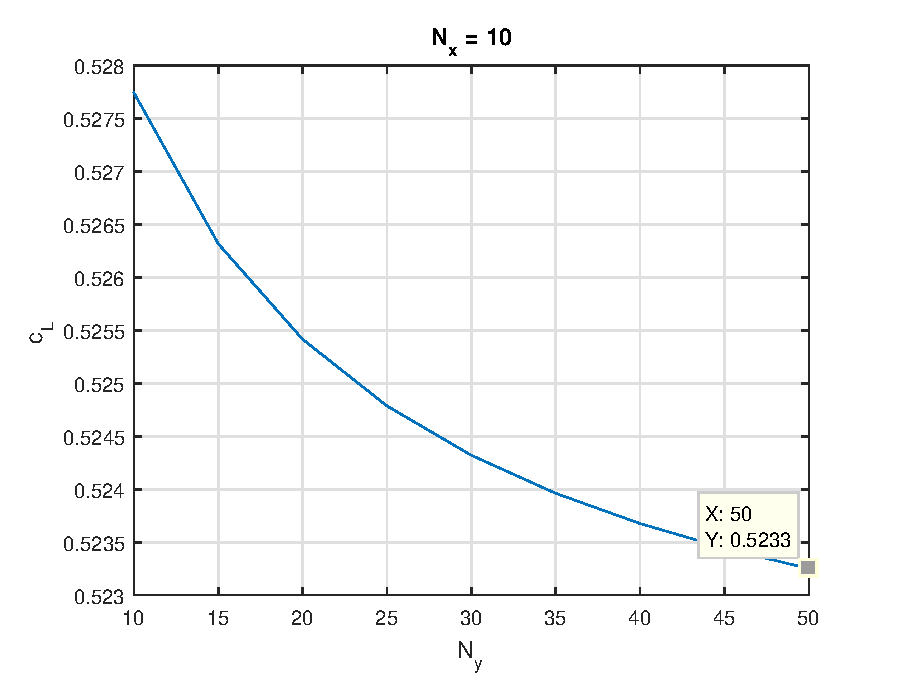
\includegraphics{./plots/nycl}
	\caption{Estudi del nombre de divisions al llarg de l'eix Y}
	\label{ny}
\end{figure}

Com es pot observar, el coeficient de sustentació tendeix a un valor de $C_{L}=0.523$. No obstant, amb 10 panells s'obté $C_{L}=0.5277$, valor que només es desvia un $0.86\%$. És a dir, que aquest nombre de divisions ja és suficient per tal d'obtenir uns valors acurats. Tanmateix, a mesura que s'augmenten els panells aquest error disminueix considerablement.

Cal tenir en compte que el número que expressa el valor $N_{y}$ són els panells en una semi-ala, per tant, el nombre total de divisions en l'eix Y és el doble.

S'ha executat el mateix anàlisi per a l'eix X, en aquest cas mantenint constant el número de panells al llarg de l'ala ($N_{y}=30$). Els resultats obtinguts es troben a la figura \ref{nx}.

\begin{figure}[h]
	\centering
	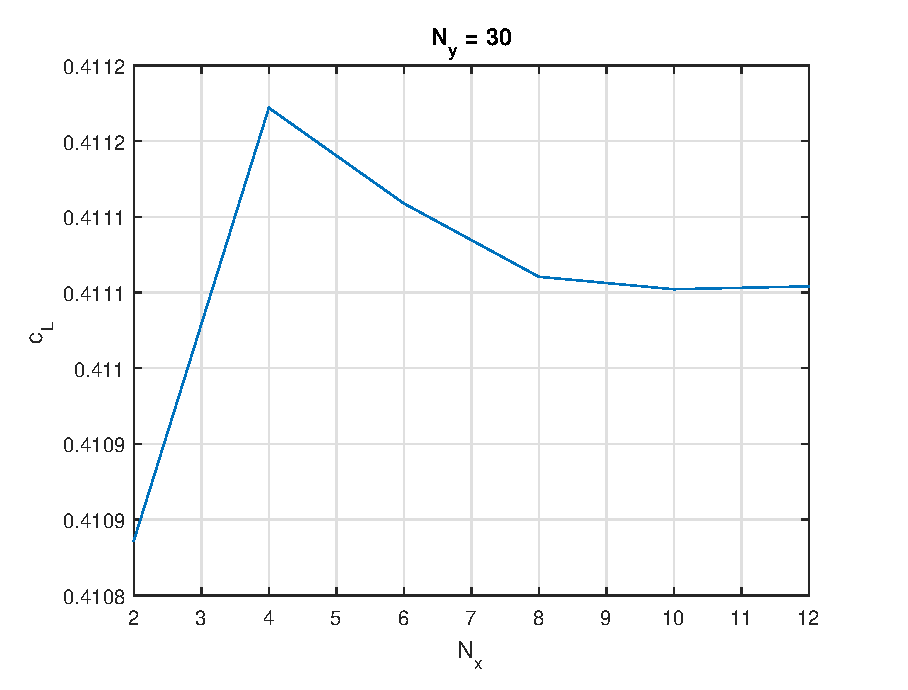
\includegraphics{./plots/nxcl}
	\caption{Estudi del nombre de divisions al llarg de l'eix X}
	\label{nx}
\end{figure}

En quant als resultats, es s'observa com la sustentació tendeix a un valor de $C_{L}=0.5243$, valor molt semblant a l'obtingut anteriorment. Comparant el diferent número de panells, s'observa com en el cas de 2 l'error és de $0.04\%$, però a partir d'aquí ja va disminuint.

Tenint en compte tots aquests resultats, s'ha optat per realitzar els càlculs que es troben en aquest informe amb un nombre de divisions $N_{x}=5$ i $N_{y}=10$.

\newpage
miau miau miau
\begin{figure}[h]
		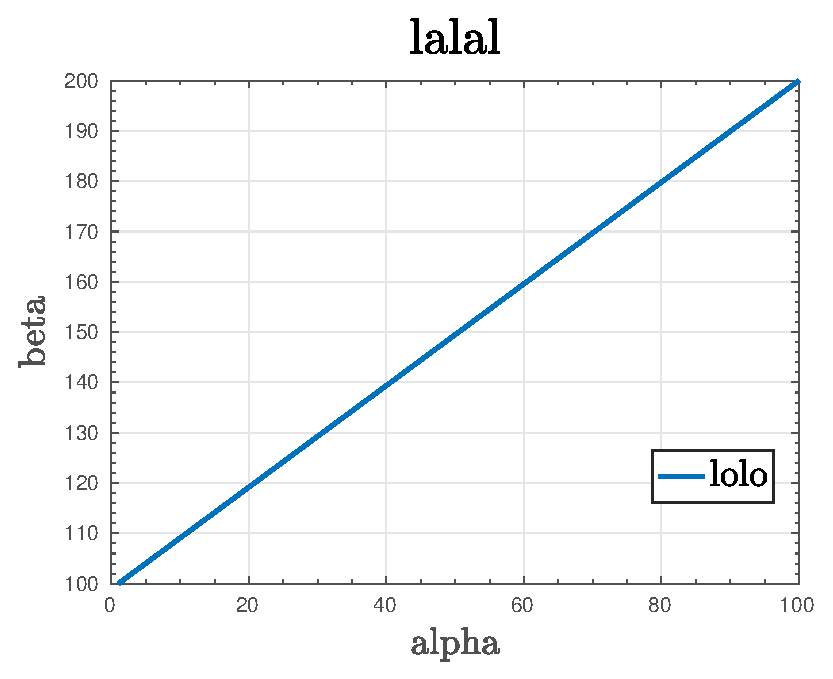
\includegraphics[width=\textwidth]{./plots/test}
		\caption{bau bau}
\end{figure}
